\documentclass{article}
\usepackage{lmodern}
\usepackage[utf8]{inputenc}
\usepackage[british]{babel}
\usepackage{geometry}
\usepackage{color}
\usepackage{amsfonts}
\usepackage{amsmath}
\usepackage{amssymb}
\usepackage{amsthm}
\usepackage{graphicx}
\usepackage{mathtools}
\usepackage{listings}
\usepackage{newlfont}
\usepackage{tikz-cd}
\usepackage{rotating}
\usepackage[backend=biber]{biblatex}
\bibliography{~/math/references.bib}

\newcommand{\numberset}{\mathbb}
\newcommand{\N}{\numberset{N}}
\newcommand{\Z}{\numberset{Z}}
\newcommand{\R}{\numberset{R}}
\newcommand{\Q}{\numberset{Q}}
\newcommand{\K}{\numberset{K}}
\newcommand{\F}{\numberset{F}}
\newcommand{\n}{\mathcal{N}}
\newcommand{\aid}{\mathfrak{a}}
\newcommand{\bid}{\mathfrak{b}}
\newcommand{\pid}{\mathfrak{p}}
\newcommand{\qid}{\mathfrak{q}}
\newcommand{\mi}{\mathfrak{m}}
\newcommand{\I}{\mathbb{I}}
\newcommand{\V}{\mathbb{V}}
\newcommand{\A}{\mathbb{A}}
\newcommand{\Ps}{\mathbb{P}}
\newcommand{\exercise}[1]{\noindent {\bf Exercise #1}}

\DeclareMathOperator{\Ima}{Im}
\DeclareMathOperator{\coker}{coker}
\DeclareMathOperator{\Id}{Id}
\DeclareMathOperator{\GL}{GL}
\DeclareMathOperator{\Mat}{Mat}

\begin{document}

\title{Representation Theory of Finite Groups - Assignment 1}

\author{Matteo Durante, s2303760, Leiden University}

\maketitle


~\\
\exercise{1.5}

Let $L=\{l_1,\ldots,l_4\}$ be the set of diagonals linking opposite vertices of
a cube. We will show that the action of $G$ on $L$ is like the one of $S_4$ on
$\{1,\ldots,4\}$.
\begin{figure}[h!]
    \centering
    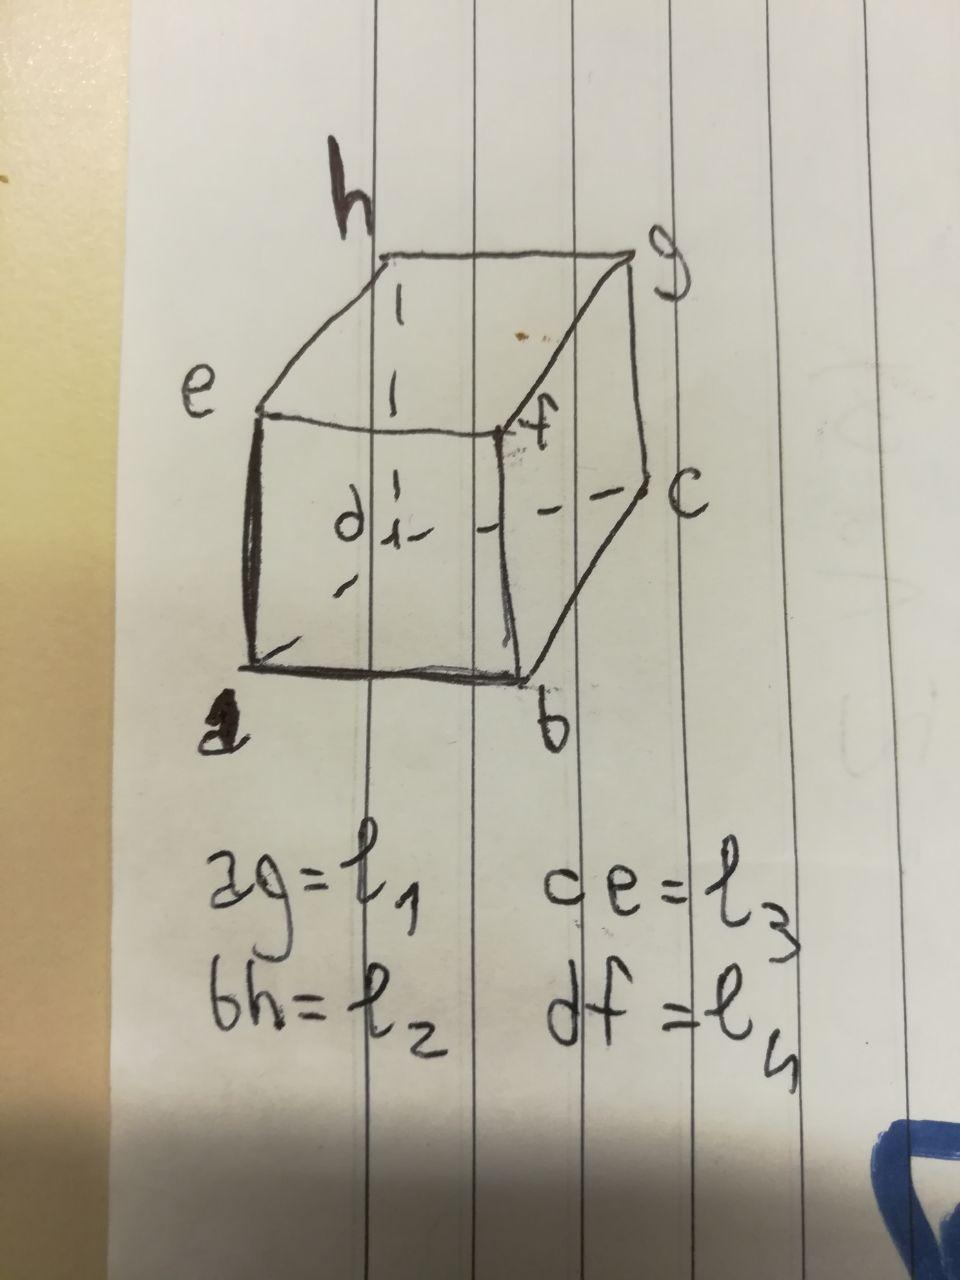
\includegraphics[width=4.0cm]{photo_2019-02-17_23-02-40.jpg}
\end{figure}

We will do so by defining an epimorphism $G\xrightarrow{\phi} S(L)\subset
S_4$, where $\sigma\in G$ is sent to an element of $S(L)\subset S_4$ obtained by
substituting a vertex $a$ with the diagonal it belongs to in the representation
of $\sigma$. This will induce an isomorphism $G/\ker(\phi)\cong S(L)$, which
will be $=S_4$, and by cardinality $\ker(\phi)$ will be a subgroup of $G$ 
of order 2 (*). $S_4$ is solvable, as the chain $S_4\supset A_4\supset K_4
\supset \{\Id\}$ shows ($K_4\cong\Z/2\Z\times\Z/2\Z$), while 
$\ker(\phi)\cong\Z/2\Z$ is abelian and hence solvable.

The only thing we need to argue is that $S(L)=S_4$. We only have
to show that we can get the elements $\{(1,2),(2,3),(3,4),(1,4)\}$, which
generate $S_4$. Consider the
transposition $\tau=(1,2)$ (for the others, the procedure is identical by
symmetry). We want a $\sigma\in G$ which would swap $l_1$ and $l_2$ while
leaving $l_3$ and $l_4$ where they are. To do this, consider the plane $P_{3,4}$ in
which $l_3$ and $l_4$ lie and observe that, with respect to this plane, $l_1$
and $l_2$ are symmetric. Take then the transformation $\sigma$ given by
the reflection with respect to this plane. This is precisely what we wanted.

We will now, thanks to this, construct the desired chain of subgroups of
$G$.

Remember that (*) $\ker(\phi)\cong\Z/2\Z$, as $|G|=48$, $|S_4|=24$ and
$|G|=|S_4|\cdot |\ker(\phi)|$. Since $G/\ker(\phi)\cong S_4$ is solvable and the same
goes for $\ker(\phi)$, looking at the preimages of the groups in the previously
identified resolution of $S_4$, we have that:
\begin{align*}
    G/\phi^{-1}(A_4) &\cong(G/\ker(\phi))/(\phi^{-1}(A_4)/\ker(\phi))\cong S_4/A_4 \\
    \phi^{-1}(A_4)/\phi^{-1}(K_4) &\cong
    (\phi^{-1}(A_4)/\ker(\phi))/(\phi^{-1}(K_4)/\ker(\phi))\cong A_4/K_4 \\
    \phi^{-1}(K_4)/\ker(\phi) &\cong K_4 \\
    \ker(\phi)/\{\Id\} &\cong\ker(\phi)
\end{align*}

It follows that
$G\supset\phi^{-1}(A_4)\supset\phi^{-1}(K_4)\supset\ker(\phi)\supset
\{\Id\}$ is a resolution of $G$.



~\\
\exercise{1.13}

First of all, let $f\in End_R(M)$, where $M$ is a $R$-module.  Then, for any 
$a\in A$ and any $m\in i^*M$, we have that $f(a\cdot m)=f(i(a)\cdot m)=i(a)\cdot 
f(m)=a\cdot f(m)$, i.e. $f$ naturally defines a $A$-module endomorphism on 
$i^*M$, hence we have a natural ring homomorphism (actually, an inclusion) $End_R(M)
\hookrightarrow End_A(i^*M)$. The $R$-module structure on $M$ uniquely defines a 
ring homomorphism $R\rightarrow End_R(M)$, which can then be composed to get the 
desired ring homomorphism $R\rightarrow End_A(i^*M)$.


~\\
\exercise{2.4}

$(3\Rightarrow 1,2)$ Trivial, as the natural arrows $N\xrightarrow{i'} L\oplus N$, 
$L\oplus N\xrightarrow{p'} L$ are s.t. $p\circ i'=\Id_N$ and $p_L\circ i=\Id_L$,
hence we may define $r:=p'\circ h$, $s:=h^{-1}\circ i'$, which will then satisfy 
$r\circ f=p'\circ h\circ f=p'\circ i=\Id_L$ and $g\circ s=g\circ h^{-1}\circ i'=
p\circ i'=\Id_N$.

$(1\Rightarrow 3)$ Let's set $P:=i\circ r$ and let $m\in M$. Such an element can be 
decomposed as $m=(m-P(m))+P(m)$, where $m-P(m)\in\ker(r)$ and $P(m)\in\Ima(i)$ 
by construction. Indeed, $r(m-P(m))=r(m)-r(i(r(m)))=r(m)-r(m)=0$.

If $m=m'+m''$, where $m'\in\ker(r), m''\in\Ima(i)$, then $m'-(m-P(m))=P(m)-m''\in
\ker(r)\cap\Ima(i)$ and, if for some $m\in M$ we have $m=i(l), 0=r(m)$, then
$0=r(m)=r(i(l))=l$, i.e. $m'=m-P(m)$ and $m''=P(m)$. It follows that the 
decomposition is unique, hence $M\cong \Ima(i)\oplus\ker(r)$. 

By exactness, $\Ima(i)\cong L$ and $M/\Ima(i)\cong\ker(r)\cong\Ima(p)=N$, thus 
$M\cong L\oplus N$.

$(2\Rightarrow 3)$ Let's set $P=s\circ p$ and let $m\in M$. Such an element can be 
decomposed as $m=(m-P(m))+P(m)$, where $m-P(m)\in\ker(p)$ and $P(m)\in\Ima(s)$ 
by construction. Indeed, $p(m-P(m))=p(m)-p(s(p(m)))=p(m)-p(m)=0$.

If $m=m'+m''$, where $m'\in\ker(p), m''\in\Ima(s)$, then $m'-(m-P(m))=P(m)-m''\in
\ker(p)\cap\Ima(s)$ and, if for some $m\in M$ we have $m=s(n), 0=p(m)$, then
$0=p(m)-p(s(n))=n$, i.e. $m'=m-P(m)$ and $m''=P(m)$. It follows that the
decomposition is unique, hence $M\cong \Ima(s)\oplus\ker(p)$.

By exactness, $\ker(p)=\Ima(i)\cong L$ and $M/\ker(p)\cong\Ima(p)=N$, thus 
$M\cong L\oplus N$.


~\\
\exercise{2.10}

$(a)$ Consider a non-zero $R$-submodule of $\K^n$, $N$. It will contain a vector 
$v\neq (0,\ldots,0)$. We may then construct a $\K$-basis of $\K^n$ containing $v$
as first element and, for any ordering of the canonical basis of $\K^n$, get an 
automorphism of $\K^n$  (the base change automorphism) sending $v$ to the first 
element of the reordered canonical basis. We have shown that, for every $i$, we 
can get a matrix $M\in\GL(n,\K)\subset\Mat(n,\K)$ s.t. $Mv=e_i$. It follows 
that, for every $i$, $e_i\in N$.

$(b)$ Consider the following homomorphism of additive abelian groups:
\begin{align*}
    f: \Mat(n,\K) &\rightarrow \K^n \\
    (a_{i,j})_{i,j=1}^n &\mapsto (a_{i,1})_{i=1}^n
\end{align*}

This is clearly surjective and, since $\Mat(n,\K)/\ker(f)\cong\K^n$, if we could
prove that $f$ is a $\Mat(n,\K)$-module homomorphism, $\ker(f)$ would be a 
maximal left ideal of $\Mat(n,\K)$. Indeed, if for $A,B\in\Mat(n,\K)$ we had 
$B\in\ker(f)$, then $f(A\cdot B)=A\cdot f(B)=A\cdot 0=0$, i.e. $A\cdot B\in\ker(f)$,
i.e. $\ker(f)$ would be a left ideal. Furthermore, $\K^n$ is a simple 
$\Mat(n,\K)$-module, whence the maximality.

Let now $A,B\in\Mat(n,\K)$ and notice the following:
\begin{align*}
    f(A\cdot B) &=f\left(\left(\sum_{k=1}^n a_{i,k}b_{k,j}\right)_{i,j=1}^n\right) \\
    &=\left(\sum_{k=1}^n a_{i,k}b_{k,1}\right)_{i=1}^n \\
    &=A\cdot (b_{k,1})_{k=1}^n \\
    &=A\cdot f(B)
\end{align*}

This shows the claim, hence the thesis. The elements of $\ker(f)$ are precisely 
the matrices whose first column is $(0)_{i=1}^n$.

\printbibliography

\end{document}
